\documentclass[11pt]{book}
\usepackage{gvv-book}
\usepackage{gvv}
\usepackage[sectionbib,authoryear]{natbib}
\setcounter{secnumdepth}{3}
\setcounter{tocdepth}{2}
\makeindex

\begin{document}
\frontmatter
\tableofcontents
\setcounter{page}{1}
\mainmatter
\chapter{Triangle}
Consider a triangle with vertices
\begin{align}
\label{eq:tri-pts}
\vec{A}=\myvec{1 \\ 0},\,
\vec{B}=\myvec{5\\4},\,
	\vec{c}=\myvec{-4\\0},\,
\end{align}

\section{Vectors}
\section{median}


\begin{enumerate}[label=\thesection.\arabic*.,ref=\thesection.\theenumi]
\numberwithin{equation}{enumi}

%Question 1.2.1:
\item  If $\vec{D}$ divides $BC$ in the ratio $k : 1$,
		\begin{align}
			\vec{D}= \frac{k\vec{C}+\vec{B}}{k+1}
		\end{align}
Find the mid points $\vec{D}, \vec{E}, \vec{F}$ of the sides $BC, CA$ and $AB$ respectively.\\
If $\vec{D}$ divides $BC$ in the ratio $k : 1$,
\begin{align}
\vec{D}= \frac{k\vec{C}+\vec{B}}{k+1}
\end{align}
Find the mid points $\vec{D}, \vec{E}, \vec{F}$ of the sides $BC, CA$ and $AB$ respectively.
\newline
Given:
\begin{align}
\vec{A} &= \myvec{-3\\0\\}\\
\vec{B} &= \myvec{4\\2\\}\\
\vec{C} &= \myvec{1\\4\\}
\end{align}

\solution
Since $\vec{D}$ is the midpoint of $BC$,
\begin{align}
k &= 1\\
\implies \vec{D} &= \frac{\vec{C} + \vec{B}}{2}\\
&= \frac{1}{2}\myvec{5\\6}
\end{align}
Similarly,
\begin{align}
\vec{E} &= \frac{\vec{A} + \vec{C}}{2}\\
&= \frac{1}{2}\myvec{-2\\4}\\
\vec{F} &= \frac{\vec{A} + \vec{B}}{2}\\
&= \myvec{1/2\\1}
\end{align} 

%Question 1.2.2:
\item Find the equations of $AD, BE$ and $CF$.\\
\\ \solution:
$\vec{D}$,$\vec{E}$,$\vec{F}$ are the midpoints of $BC$,$CA$,$AB$ respectively, then\\
\begin{align}
 \vec{D} &=  \myvec{\frac{5}{2}\\3}\\
 \vec{E} &=  \myvec{-1\\2}\\
 \vec{F} &= \myvec{1/2\\1}
\end{align}
\begin{enumerate}

 \item The normal equation for the median $AD$ is
  \begin{align}
    \vec{n}^{\top}\myvec{\vec{x}-\vec{A}}&=0\\
    \implies
    \vec{n}^{\top}\vec{x}&=\vec{n}^{\top}\vec{A}
  \end{align}
 We have to find the $\vec{n}$ so that we can find $\vec{n}^{\top}$.
 Since,
\begin{align}
  \vec{n} &= \myvec{0 & 1\\
  -1 & 0}\vec{m}
\end{align}
Here $\vec{m} = \vec{D}- \vec{A}$ for median $AD$
\begin{align}
\vec{m}&=\myvec{\frac{11}{2}\\3}
\end{align}
Since,
\begin{align}
  \vec{n} &= \myvec{0 & 1\\
  -1 & 0}\vec{m}\\
\implies
\vec{n} &= \myvec{0 & 1\\
  -1 & 0}\myvec{\frac{11}{2}\\3}\\
        &= \myvec{3 \\\frac{-11}{2}}
\end{align}
Hence the normal equation of median $AD$ is 
\begin{align}
    \myvec{3 & \frac{-11}{2}}\vec{x}&=\myvec{3 & \frac{-11}{2}}\myvec{-3\\0}\\
    \implies
    \myvec{3 & \frac{-11}{2}}\vec{x}&={-9}
\end{align}

\item The normal equation for the median $BE$ is
\begin{align}
\vec{n}^{\top}\myvec{\vec{x}-\vec{B}}&=0\\
\implies
\vec{n}^{\top}\vec{x}&=\vec{n}^{\top}\vec{B}
\end{align}
Here $\vec{m} = \vec{E}- \vec{B}$ for median $BE$
\begin{align}
\vec{m}&&=\myvec{-5\\0}
\end{align}
Since,
\begin{align}
  \vec{n} &= \myvec{0 & 1\\
  -1 & 0}\vec{m}\\
\implies
\vec{n} &= \myvec{0 & 1\\
  -1 & 0}\myvec{-5\\0}\\
        &= \myvec{0\\ 5}
\end{align}
Hence the normal equation of median $BE$ is 
\begin{align}
    \myvec{0 & 5}\vec{x}&=\myvec{0 & 5}\myvec{4\\2}\\
\implies
    \myvec{0 & 5}\vec{x}&={10}
\end{align}

\item The normal equation for the median $CF$ is
\begin{align}
\vec{n}^{\top}\myvec{\vec{x}-\vec{C}}&=0\\
\implies
\vec{n}^{\top}\vec{x}&=\vec{n}^{\top}\vec{C}
\end{align}
Here $\vec{m} = \vec{F}- \vec{C}$ for median $CF$
\begin{align}
\vec{m}&=\myvec{\frac{-1}{2}\\-3}
\end{align}
Since,
\begin{align}
  \vec{n} &= \myvec{0 & 1\\
  -1 & 0}\vec{m}\\
\implies
\vec{n} &= \myvec{0 & 1\\
  -1 & 0}\myvec{\frac{-1}{2} \\ -3 }\\
        &= \myvec{-3 \\ \frac{1}{2}}
\end{align}
Hence the normal equation of median $CF$ is 
\begin{align}
    \myvec{-3 & \frac{1}{2} }\vec{x}&=\myvec{-3 & \frac{1}{2}}\myvec{1\\4}\\
\implies
    \myvec{-3 & \frac{1}{2}}\vec{x}&=-1
\end{align}
\end{enumerate}

%Question 1.2.3:
\item Find the intersection $\vec{G}$ of $BE$ and $CF$
\\ 
\solution 
$\vec{A},\vec{B}$ and $\vec{C}$ are vertices of triangle:
\begin{align}
    \vec{A} &= \myvec-3 \\0} \\
    \vec{B} &= \myvec{4\\ 2} \\
    \vec{C} &= \myvec{1 \\4}
\end{align}
Since $\vec{E}$ and $\vec{F}$ are midpoints of $CA$ and $AB$,
\begin{align}
    \vec{E} &= \frac{\vec{A} + \vec{C}}{2} \\
	&= \myvec{-1 \\2}\\
    \vec{F} &= \frac{\vec{B} + \vec{A}}{2} \\ 
    &= \myvec{ \frac{1}{2} \\ 1}
\end{align}
The line $BE$ in vector form is given by
\begin{align}
\myvec{0 & 5} \vec{x} &= \myvec{10}
\label{eq:1.2.3,8}
\end{align}
The line $CF$ in vector form is given by
\begin{align}
\myvec{ -3&-\frac{1}{2}} \vec{x} &= \myvec{-1}
\label{eq:1.2.3,9}
\end{align}
From \eqref{eq:1.2.3,8} and \eqref{eq:1.2.3,9} the augmented matrix is:
\begin{align}
\myvec{
0 & 5 & {10} \\
-3 & \frac{1}{2} & -1
}
\end{align}
Solve for $\vec{x}$ using Gauss-Elimination method:
\begin{align}
    \label{eq:matrowoperations}
    \myvec{
    1 & 0 & \frac{2}{3}
    \\
    0 & 1 & 2
    }
\end{align} 
Therefore, 
\begin{align}
\vec{G} = \myvec{\frac{2}{3} \\ 2}
\end{align}
From Fig. \ref{fig:Triangle101}, We can see that $\vec{G}=\myvec{\frac{2}{3}\\ 2}$ is the intersection of $BE$ and $CF$
\begin{figure}[h]
\centering
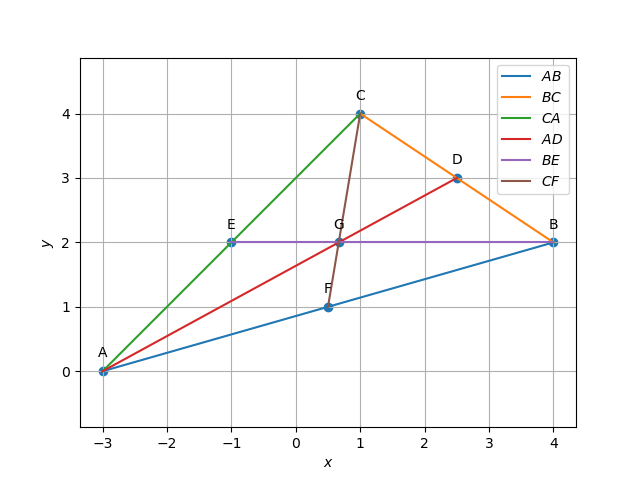
\includegraphics[width=\columnwidth]{/sdcard/geometry/geometry/figs/med2.png}
\caption{$G$ is the centroid of triangle $ABC$}
\label{fig:Triangle101}
\end{figure}



%Question 1.2.4:
\item Verify that 
		\begin{align}
			\frac{BG}{GE} = 
			\frac{CG}{GF} =
			\frac{AG}{GD} =2 
		\end{align}\\
Question 1.2.4:Verify that 
\begin{align}
		\frac{BG}{GE} = 
		\frac{CG}{GF} =
		\frac{AG}{GD} = 2 
\end{align}
\solution In order to verify the above equation we first need to find $\vec{G}$.$\vec{G}$ is the intersection of $BE$ and $CF$,Using the value of $\vec{G}$ from (1.2.3).
\begin{align}
		\vec{G} = \myvec{\frac{2}{3}\\2}
\end{align}
Also,We know that $\vec{D}, \vec{E}$ and $\vec{F}$ are midpoints of $BC, CA$ and $AB$ respectively from (1.2.1).
\begin{align}
		\vec{D} = \myvec{\frac{5}{2} \\ 3},\,
		\vec{E} = \myvec{-1 \\ 2},\,
		\vec{F} = \myvec{\frac{1}{2}\\ 1}
\end{align}
\begin{enumerate}
\item Calculating the ratio of $BG$ and $GE$,
\begin{align}
		\label{eq:tri-pts/4} \vec{G}-\vec{B} &= \myvec{\frac{-10}{3} \\ 0} \\
		\label{eq:tri-pts/5} \vec{E}-\vec{G} &= \myvec{\frac{-5}{3} \\ 0} \\
		\label{eq:tri-pts/6} \norm{\vec{G}-\vec{B}} &= \sqrt{\brak{\frac{-10}{0}}^2 + \brak{\frac{-5}{0}}^{2}}  \\
		\label{eq:tri-pts/7} \norm{\vec{E}-\vec{G}} &= \sqrt{\brak{\frac{-13}{6}}^2 + \brak{\frac{-4}{3}}^2} &= \frac{\sqrt{233}}{6} \\
		\label{eq:tri-pts/8}\frac{BG}{GE} &= \frac{\norm{\vec{G}-\vec{B}}}{\norm{\vec{E}-\vec{G}}}&= 2  
\end{align}		
\end{enumerate}

From \eqref{eq:tri-pts/8}, \eqref{eq:tri-pts/13}, \eqref{eq:tri-pts/18}
\begin{align}
		\frac{BG}{GE} = 
		\frac{CG}{GF} =
		\frac{AG}{GD} = 2
\end{align}
Hence verified.



%Question 1.2.5:
\item Show that $\vec{A}, \vec{G}$ and $\vec{D}$ are collinear.\\
\solution 
Given that,
\begin{align}
    \vec{A} = \myvec{-3\\0}
    \quad
    \vec{B} &= \myvec{4\\2}
    \quad
    \vec{C} = \myvec{1\\4}
\end{align}
We need to show that points $\vec{A},\vec{D},\vec{G}$ are collinear.
From Problem 1.2.3 We know that, The point $\vec{G}$ is 
\begin{align}
    \vec{G} &=\myvec{\frac{2}{3}\\ 2}
\end{align}
And from Problem 1.2.1 We know that, The point $\vec{D}$ is 
\begin{align}
    \vec{D} &=\myvec{\frac{5}{2}\\ 3}
\end{align}
In Problem 1.1.3, There is a theorem/law mentioned i.e.,

Points $\vec{A},\vec{D},\vec{G}$ are defined to be collinear if 
\begin{align}
    \text{rank}\myvec{
    1 & 1 & 1\\
    \vec{A} & \vec{D} & \vec{G} \\
    } &= 2 
\end{align} 
Using the above law/Theorem Let
\begin{align}
    \vec{R}&=\myvec{
    1 & 1 & 1
    \\
    -3 & \frac{5}{2} & \frac{2}{3}
    \\
    0 & 3 & 2
    } 
\end{align} 
The matrix $\vec{R}$ can be row reduced as follows,
\begin{align}
    \label{eq:mat_row_operations}
    \myvec{
    1 & 1 & 1
    \\
    -3 & \frac{5}{2} & \frac{2}{3}
    \\
    0 & 3 & 2
    }
     \xleftrightarrow[]{}
    \myvec{
    1 & 1 & 1
    \\
    0 & 1 & \frac{2}{3}
    \\
    0 & 0 & 0
    }
\end{align}
Rank of above matrix is 2.\\
Hence, we proved that that points $\vec{A},\vec{D},\vec{G}$ are collinear.



%Question 1.2.6:
\item Verify that 
		\begin{align}
			\vec{G}=\frac{\vec{A}+\vec{B}+\vec{C}}{3}
		\end{align}
$\vec{G}$ is known as the {\em centroid} of $\triangle ABC$.\\
Verify that\\
\begin{align}
 \vec{G}=\frac{\vec{A}+\vec{B}+\vec{C}}{3}   
\end{align}
$\vec{G}$ is known as the \underline{centroid} of $\triangle$ABC 
SOLUTION:\\
let us first evaluate the R.H.S of the equation
\begin{equation}
\begin{split}
\label{eq:centroid}
    \vec{G}&= \frac{\myvec{-3\\0}+\myvec{4\\2}+\myvec{1\\4}}{3}\\   
     &= \myvec{\frac{2}{3}\\ 2}
\end{split}
\end{equation}
Hence verified.


%Question 1.2.7: 
\item Verify that 
		\begin{align}
\vec{A}-\vec{F}=\vec{E}-\vec{D}
		\end{align}
The quadrilateral $AFDE$ is defined to be a parallelogram.\\
Question : Verify that 
\begin{align}
	\vec{A}-\vec{F} = \vec{E}-\vec{D}
\end{align}
The quadrilateral $AFDE$ is defined to be parallelogram
\\ \solution 
Given that,
\begin{align}
    \vec{A} = \myvec{-3\\0}
    \quad
    \vec{B} &= \myvec{4\\2}
    \quad
    \vec{C} = \myvec{1\\4}
\end{align}
From Problem 1.2.1 We know that, The point $\vec{D},\vec{E},\vec{F}$ is 
\begin{align}
    \vec{D} = \myvec{\frac{5}{2}\\ 3 }
    \quad
    \vec{E} &= \myvec{-1\\2}
    \quad
    \vec{F} = \myvec{\frac{1}{2}\\ 1}
\end{align}
Evaluating the R.H.S of the equation
\begin{align}
    \vec{A}-\vec{F}&=\myvec{ \frac{-7}{2} \\ -1 }
\end{align} 
Evaluating the L.H.S of the equation
\begin{align}
    \vec{E}-\vec{D}&=\myvec{\frac{-7}{2} \\ -1 }
\end{align}
Hence verified that, R.H.S = L.H.S i.e.,
\begin{align}
	\vec{A}-\vec{F} = \vec{E}-\vec{D}
\end{align}
From the fig\ref{fig:Triangle}, It is verified that $AFDE$ is a parallelogram
\begin{figure}
\centering
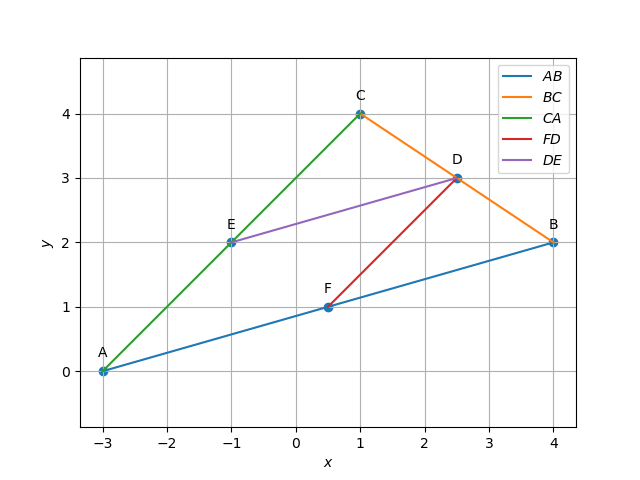
\includegraphics[width=\columnwidth]{/sdcard/geometry/geometry/figs/prm.png}
\caption{$AFDE$ form a parallelogram in triangle ABC}
\label{fig:Triangle}
\end{figure}
\end{enumerate}














%\documentclass[11pt]{book}
\usepackage{gvv-book}
\usepackage{gvv}
\usepackage[sectionbib,authoryear]{natbib}
\setcounter{secnumdepth}{3}
\setcounter{tocdepth}{2}
\makeindex

\begin{document}
\frontmatter
\tableofcontents
\setcounter{page}{1}
\mainmatter
\chapter{Triangle}
Consider a triangle with vertices
\begin{align}
\label{eq:tri-pts}
\vec{A}=\myvec{1 \\ 0},\,
\vec{B}=\myvec{5\\4},\,
	\vec{c}=\myvec{-4\\0},\,
\end{align}

\section{Vectors}
\section{median}


\begin{enumerate}[label=\thesection.\arabic*.,ref=\thesection.\theenumi]
\numberwithin{equation}{enumi}

%Question 1.2.1:
\item  If $\vec{D}$ divides $BC$ in the ratio $k : 1$,
		\begin{align}
			\vec{D}= \frac{k\vec{C}+\vec{B}}{k+1}
		\end{align}
Find the mid points $\vec{D}, \vec{E}, \vec{F}$ of the sides $BC, CA$ and $AB$ respectively.\\
If $\vec{D}$ divides $BC$ in the ratio $k : 1$,
\begin{align}
\vec{D}= \frac{k\vec{C}+\vec{B}}{k+1}
\end{align}
Find the mid points $\vec{D}, \vec{E}, \vec{F}$ of the sides $BC, CA$ and $AB$ respectively.
\newline
Given:
\begin{align}
\vec{A} &= \myvec{-3\\0\\}\\
\vec{B} &= \myvec{4\\2\\}\\
\vec{C} &= \myvec{1\\4\\}
\end{align}

\solution
Since $\vec{D}$ is the midpoint of $BC$,
\begin{align}
k &= 1\\
\implies \vec{D} &= \frac{\vec{C} + \vec{B}}{2}\\
&= \frac{1}{2}\myvec{5\\6}
\end{align}
Similarly,
\begin{align}
\vec{E} &= \frac{\vec{A} + \vec{C}}{2}\\
&= \frac{1}{2}\myvec{-2\\4}\\
\vec{F} &= \frac{\vec{A} + \vec{B}}{2}\\
&= \myvec{1/2\\1}
\end{align} 

%Question 1.2.2:
\item Find the equations of $AD, BE$ and $CF$.\\
\\ \solution:
$\vec{D}$,$\vec{E}$,$\vec{F}$ are the midpoints of $BC$,$CA$,$AB$ respectively, then\\
\begin{align}
 \vec{D} &=  \myvec{\frac{5}{2}\\3}\\
 \vec{E} &=  \myvec{-1\\2}\\
 \vec{F} &= \myvec{1/2\\1}
\end{align}
\begin{enumerate}

 \item The normal equation for the median $AD$ is
  \begin{align}
    \vec{n}^{\top}\myvec{\vec{x}-\vec{A}}&=0\\
    \implies
    \vec{n}^{\top}\vec{x}&=\vec{n}^{\top}\vec{A}
  \end{align}
 We have to find the $\vec{n}$ so that we can find $\vec{n}^{\top}$.
 Since,
\begin{align}
  \vec{n} &= \myvec{0 & 1\\
  -1 & 0}\vec{m}
\end{align}
Here $\vec{m} = \vec{D}- \vec{A}$ for median $AD$
\begin{align}
\vec{m}&=\myvec{\frac{11}{2}\\3}
\end{align}
Since,
\begin{align}
  \vec{n} &= \myvec{0 & 1\\
  -1 & 0}\vec{m}\\
\implies
\vec{n} &= \myvec{0 & 1\\
  -1 & 0}\myvec{\frac{11}{2}\\3}\\
        &= \myvec{3 \\\frac{-11}{2}}
\end{align}
Hence the normal equation of median $AD$ is 
\begin{align}
    \myvec{3 & \frac{-11}{2}}\vec{x}&=\myvec{3 & \frac{-11}{2}}\myvec{-3\\0}\\
    \implies
    \myvec{3 & \frac{-11}{2}}\vec{x}&={-9}
\end{align}

\item The normal equation for the median $BE$ is
\begin{align}
\vec{n}^{\top}\myvec{\vec{x}-\vec{B}}&=0\\
\implies
\vec{n}^{\top}\vec{x}&=\vec{n}^{\top}\vec{B}
\end{align}
Here $\vec{m} = \vec{E}- \vec{B}$ for median $BE$
\begin{align}
\vec{m}&&=\myvec{-5\\0}
\end{align}
Since,
\begin{align}
  \vec{n} &= \myvec{0 & 1\\
  -1 & 0}\vec{m}\\
\implies
\vec{n} &= \myvec{0 & 1\\
  -1 & 0}\myvec{-5\\0}\\
        &= \myvec{0\\ 5}
\end{align}
Hence the normal equation of median $BE$ is 
\begin{align}
    \myvec{0 & 5}\vec{x}&=\myvec{0 & 5}\myvec{4\\2}\\
\implies
    \myvec{0 & 5}\vec{x}&={10}
\end{align}

\item The normal equation for the median $CF$ is
\begin{align}
\vec{n}^{\top}\myvec{\vec{x}-\vec{C}}&=0\\
\implies
\vec{n}^{\top}\vec{x}&=\vec{n}^{\top}\vec{C}
\end{align}
Here $\vec{m} = \vec{F}- \vec{C}$ for median $CF$
\begin{align}
\vec{m}&=\myvec{\frac{-1}{2}\\-3}
\end{align}
Since,
\begin{align}
  \vec{n} &= \myvec{0 & 1\\
  -1 & 0}\vec{m}\\
\implies
\vec{n} &= \myvec{0 & 1\\
  -1 & 0}\myvec{\frac{-1}{2} \\ -3 }\\
        &= \myvec{-3 \\ \frac{1}{2}}
\end{align}
Hence the normal equation of median $CF$ is 
\begin{align}
    \myvec{-3 & \frac{1}{2} }\vec{x}&=\myvec{-3 & \frac{1}{2}}\myvec{1\\4}\\
\implies
    \myvec{-3 & \frac{1}{2}}\vec{x}&=-1
\end{align}
\end{enumerate}

%Question 1.2.3:
\item Find the intersection $\vec{G}$ of $BE$ and $CF$
\\ 
\solution 
$\vec{A},\vec{B}$ and $\vec{C}$ are vertices of triangle:
\begin{align}
    \vec{A} &= \myvec-3 \\0} \\
    \vec{B} &= \myvec{4\\ 2} \\
    \vec{C} &= \myvec{1 \\4}
\end{align}
Since $\vec{E}$ and $\vec{F}$ are midpoints of $CA$ and $AB$,
\begin{align}
    \vec{E} &= \frac{\vec{A} + \vec{C}}{2} \\
	&= \myvec{-1 \\2}\\
    \vec{F} &= \frac{\vec{B} + \vec{A}}{2} \\ 
    &= \myvec{ \frac{1}{2} \\ 1}
\end{align}
The line $BE$ in vector form is given by
\begin{align}
\myvec{0 & 5} \vec{x} &= \myvec{10}
\label{eq:1.2.3,8}
\end{align}
The line $CF$ in vector form is given by
\begin{align}
\myvec{ -3&-\frac{1}{2}} \vec{x} &= \myvec{-1}
\label{eq:1.2.3,9}
\end{align}
From \eqref{eq:1.2.3,8} and \eqref{eq:1.2.3,9} the augmented matrix is:
\begin{align}
\myvec{
0 & 5 & {10} \\
-3 & \frac{1}{2} & -1
}
\end{align}
Solve for $\vec{x}$ using Gauss-Elimination method:
\begin{align}
    \label{eq:matrowoperations}
    \myvec{
    1 & 0 & \frac{2}{3}
    \\
    0 & 1 & 2
    }
\end{align} 
Therefore, 
\begin{align}
\vec{G} = \myvec{\frac{2}{3} \\ 2}
\end{align}
From Fig. \ref{fig:Triangle101}, We can see that $\vec{G}=\myvec{\frac{2}{3}\\ 2}$ is the intersection of $BE$ and $CF$
\begin{figure}[h]
\centering
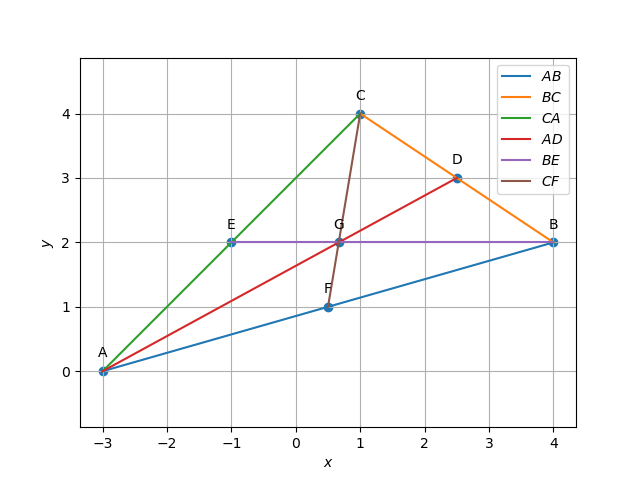
\includegraphics[width=\columnwidth]{/sdcard/geometry/geometry/figs/med2.png}
\caption{$G$ is the centroid of triangle $ABC$}
\label{fig:Triangle101}
\end{figure}



%Question 1.2.4:
\item Verify that 
		\begin{align}
			\frac{BG}{GE} = 
			\frac{CG}{GF} =
			\frac{AG}{GD} =2 
		\end{align}\\
Question 1.2.4:Verify that 
\begin{align}
		\frac{BG}{GE} = 
		\frac{CG}{GF} =
		\frac{AG}{GD} = 2 
\end{align}
\solution In order to verify the above equation we first need to find $\vec{G}$.$\vec{G}$ is the intersection of $BE$ and $CF$,Using the value of $\vec{G}$ from (1.2.3).
\begin{align}
		\vec{G} = \myvec{\frac{2}{3}\\2}
\end{align}
Also,We know that $\vec{D}, \vec{E}$ and $\vec{F}$ are midpoints of $BC, CA$ and $AB$ respectively from (1.2.1).
\begin{align}
		\vec{D} = \myvec{\frac{5}{2} \\ 3},\,
		\vec{E} = \myvec{-1 \\ 2},\,
		\vec{F} = \myvec{\frac{1}{2}\\ 1}
\end{align}
\begin{enumerate}
\item Calculating the ratio of $BG$ and $GE$,
\begin{align}
		\label{eq:tri-pts/4} \vec{G}-\vec{B} &= \myvec{\frac{-10}{3} \\ 0} \\
		\label{eq:tri-pts/5} \vec{E}-\vec{G} &= \myvec{\frac{-5}{3} \\ 0} \\
		\label{eq:tri-pts/6} \norm{\vec{G}-\vec{B}} &= \sqrt{\brak{\frac{-10}{0}}^2 + \brak{\frac{-5}{0}}^{2}}  \\
		\label{eq:tri-pts/7} \norm{\vec{E}-\vec{G}} &= \sqrt{\brak{\frac{-13}{6}}^2 + \brak{\frac{-4}{3}}^2} &= \frac{\sqrt{233}}{6} \\
		\label{eq:tri-pts/8}\frac{BG}{GE} &= \frac{\norm{\vec{G}-\vec{B}}}{\norm{\vec{E}-\vec{G}}}&= 2  
\end{align}		
\end{enumerate}

From \eqref{eq:tri-pts/8}, \eqref{eq:tri-pts/13}, \eqref{eq:tri-pts/18}
\begin{align}
		\frac{BG}{GE} = 
		\frac{CG}{GF} =
		\frac{AG}{GD} = 2
\end{align}
Hence verified.



%Question 1.2.5:
\item Show that $\vec{A}, \vec{G}$ and $\vec{D}$ are collinear.\\
\solution 
Given that,
\begin{align}
    \vec{A} = \myvec{-3\\0}
    \quad
    \vec{B} &= \myvec{4\\2}
    \quad
    \vec{C} = \myvec{1\\4}
\end{align}
We need to show that points $\vec{A},\vec{D},\vec{G}$ are collinear.
From Problem 1.2.3 We know that, The point $\vec{G}$ is 
\begin{align}
    \vec{G} &=\myvec{\frac{2}{3}\\ 2}
\end{align}
And from Problem 1.2.1 We know that, The point $\vec{D}$ is 
\begin{align}
    \vec{D} &=\myvec{\frac{5}{2}\\ 3}
\end{align}
In Problem 1.1.3, There is a theorem/law mentioned i.e.,

Points $\vec{A},\vec{D},\vec{G}$ are defined to be collinear if 
\begin{align}
    \text{rank}\myvec{
    1 & 1 & 1\\
    \vec{A} & \vec{D} & \vec{G} \\
    } &= 2 
\end{align} 
Using the above law/Theorem Let
\begin{align}
    \vec{R}&=\myvec{
    1 & 1 & 1
    \\
    -3 & \frac{5}{2} & \frac{2}{3}
    \\
    0 & 3 & 2
    } 
\end{align} 
The matrix $\vec{R}$ can be row reduced as follows,
\begin{align}
    \label{eq:mat_row_operations}
    \myvec{
    1 & 1 & 1
    \\
    -3 & \frac{5}{2} & \frac{2}{3}
    \\
    0 & 3 & 2
    }
     \xleftrightarrow[]{}
    \myvec{
    1 & 1 & 1
    \\
    0 & 1 & \frac{2}{3}
    \\
    0 & 0 & 0
    }
\end{align}
Rank of above matrix is 2.\\
Hence, we proved that that points $\vec{A},\vec{D},\vec{G}$ are collinear.



%Question 1.2.6:
\item Verify that 
		\begin{align}
			\vec{G}=\frac{\vec{A}+\vec{B}+\vec{C}}{3}
		\end{align}
$\vec{G}$ is known as the {\em centroid} of $\triangle ABC$.\\
Verify that\\
\begin{align}
 \vec{G}=\frac{\vec{A}+\vec{B}+\vec{C}}{3}   
\end{align}
$\vec{G}$ is known as the \underline{centroid} of $\triangle$ABC 
SOLUTION:\\
let us first evaluate the R.H.S of the equation
\begin{equation}
\begin{split}
\label{eq:centroid}
    \vec{G}&= \frac{\myvec{-3\\0}+\myvec{4\\2}+\myvec{1\\4}}{3}\\   
     &= \myvec{\frac{2}{3}\\ 2}
\end{split}
\end{equation}
Hence verified.


%Question 1.2.7: 
\item Verify that 
		\begin{align}
\vec{A}-\vec{F}=\vec{E}-\vec{D}
		\end{align}
The quadrilateral $AFDE$ is defined to be a parallelogram.\\
Question : Verify that 
\begin{align}
	\vec{A}-\vec{F} = \vec{E}-\vec{D}
\end{align}
The quadrilateral $AFDE$ is defined to be parallelogram
\\ \solution 
Given that,
\begin{align}
    \vec{A} = \myvec{-3\\0}
    \quad
    \vec{B} &= \myvec{4\\2}
    \quad
    \vec{C} = \myvec{1\\4}
\end{align}
From Problem 1.2.1 We know that, The point $\vec{D},\vec{E},\vec{F}$ is 
\begin{align}
    \vec{D} = \myvec{\frac{5}{2}\\ 3 }
    \quad
    \vec{E} &= \myvec{-1\\2}
    \quad
    \vec{F} = \myvec{\frac{1}{2}\\ 1}
\end{align}
Evaluating the R.H.S of the equation
\begin{align}
    \vec{A}-\vec{F}&=\myvec{ \frac{-7}{2} \\ -1 }
\end{align} 
Evaluating the L.H.S of the equation
\begin{align}
    \vec{E}-\vec{D}&=\myvec{\frac{-7}{2} \\ -1 }
\end{align}
Hence verified that, R.H.S = L.H.S i.e.,
\begin{align}
	\vec{A}-\vec{F} = \vec{E}-\vec{D}
\end{align}
From the fig\ref{fig:Triangle}, It is verified that $AFDE$ is a parallelogram
\begin{figure}
\centering
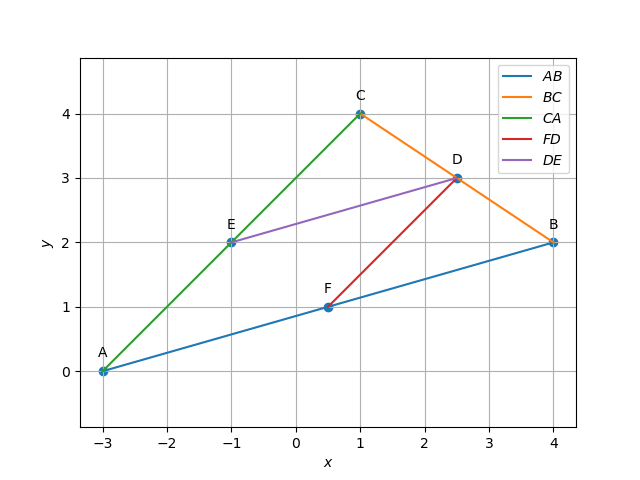
\includegraphics[width=\columnwidth]{/sdcard/geometry/geometry/figs/prm.png}
\caption{$AFDE$ form a parallelogram in triangle ABC}
\label{fig:Triangle}
\end{figure}
\end{enumerate}














%\documentclass[11pt]{book}
\usepackage{gvv-book}
\usepackage{gvv}
\usepackage[sectionbib,authoryear]{natbib}
\setcounter{secnumdepth}{3}
\setcounter{tocdepth}{2}
\makeindex

\begin{document}
\frontmatter
\tableofcontents
\setcounter{page}{1}
\mainmatter
\chapter{Triangle}
Consider a triangle with vertices
\begin{align}
\label{eq:tri-pts}
\vec{A}=\myvec{1 \\ 0},\,
\vec{B}=\myvec{5\\4},\,
	\vec{c}=\myvec{-4\\0},\,
\end{align}

\section{Vectors}
\section{median}


\begin{enumerate}[label=\thesection.\arabic*.,ref=\thesection.\theenumi]
\numberwithin{equation}{enumi}

%Question 1.2.1:
\item  If $\vec{D}$ divides $BC$ in the ratio $k : 1$,
		\begin{align}
			\vec{D}= \frac{k\vec{C}+\vec{B}}{k+1}
		\end{align}
Find the mid points $\vec{D}, \vec{E}, \vec{F}$ of the sides $BC, CA$ and $AB$ respectively.\\
If $\vec{D}$ divides $BC$ in the ratio $k : 1$,
\begin{align}
\vec{D}= \frac{k\vec{C}+\vec{B}}{k+1}
\end{align}
Find the mid points $\vec{D}, \vec{E}, \vec{F}$ of the sides $BC, CA$ and $AB$ respectively.
\newline
Given:
\begin{align}
\vec{A} &= \myvec{-3\\0\\}\\
\vec{B} &= \myvec{4\\2\\}\\
\vec{C} &= \myvec{1\\4\\}
\end{align}

\solution
Since $\vec{D}$ is the midpoint of $BC$,
\begin{align}
k &= 1\\
\implies \vec{D} &= \frac{\vec{C} + \vec{B}}{2}\\
&= \frac{1}{2}\myvec{5\\6}
\end{align}
Similarly,
\begin{align}
\vec{E} &= \frac{\vec{A} + \vec{C}}{2}\\
&= \frac{1}{2}\myvec{-2\\4}\\
\vec{F} &= \frac{\vec{A} + \vec{B}}{2}\\
&= \myvec{1/2\\1}
\end{align} 

%Question 1.2.2:
\item Find the equations of $AD, BE$ and $CF$.\\
\\ \solution:
$\vec{D}$,$\vec{E}$,$\vec{F}$ are the midpoints of $BC$,$CA$,$AB$ respectively, then\\
\begin{align}
 \vec{D} &=  \myvec{\frac{5}{2}\\3}\\
 \vec{E} &=  \myvec{-1\\2}\\
 \vec{F} &= \myvec{1/2\\1}
\end{align}
\begin{enumerate}

 \item The normal equation for the median $AD$ is
  \begin{align}
    \vec{n}^{\top}\myvec{\vec{x}-\vec{A}}&=0\\
    \implies
    \vec{n}^{\top}\vec{x}&=\vec{n}^{\top}\vec{A}
  \end{align}
 We have to find the $\vec{n}$ so that we can find $\vec{n}^{\top}$.
 Since,
\begin{align}
  \vec{n} &= \myvec{0 & 1\\
  -1 & 0}\vec{m}
\end{align}
Here $\vec{m} = \vec{D}- \vec{A}$ for median $AD$
\begin{align}
\vec{m}&=\myvec{\frac{11}{2}\\3}
\end{align}
Since,
\begin{align}
  \vec{n} &= \myvec{0 & 1\\
  -1 & 0}\vec{m}\\
\implies
\vec{n} &= \myvec{0 & 1\\
  -1 & 0}\myvec{\frac{11}{2}\\3}\\
        &= \myvec{3 \\\frac{-11}{2}}
\end{align}
Hence the normal equation of median $AD$ is 
\begin{align}
    \myvec{3 & \frac{-11}{2}}\vec{x}&=\myvec{3 & \frac{-11}{2}}\myvec{-3\\0}\\
    \implies
    \myvec{3 & \frac{-11}{2}}\vec{x}&={-9}
\end{align}

\item The normal equation for the median $BE$ is
\begin{align}
\vec{n}^{\top}\myvec{\vec{x}-\vec{B}}&=0\\
\implies
\vec{n}^{\top}\vec{x}&=\vec{n}^{\top}\vec{B}
\end{align}
Here $\vec{m} = \vec{E}- \vec{B}$ for median $BE$
\begin{align}
\vec{m}&&=\myvec{-5\\0}
\end{align}
Since,
\begin{align}
  \vec{n} &= \myvec{0 & 1\\
  -1 & 0}\vec{m}\\
\implies
\vec{n} &= \myvec{0 & 1\\
  -1 & 0}\myvec{-5\\0}\\
        &= \myvec{0\\ 5}
\end{align}
Hence the normal equation of median $BE$ is 
\begin{align}
    \myvec{0 & 5}\vec{x}&=\myvec{0 & 5}\myvec{4\\2}\\
\implies
    \myvec{0 & 5}\vec{x}&={10}
\end{align}

\item The normal equation for the median $CF$ is
\begin{align}
\vec{n}^{\top}\myvec{\vec{x}-\vec{C}}&=0\\
\implies
\vec{n}^{\top}\vec{x}&=\vec{n}^{\top}\vec{C}
\end{align}
Here $\vec{m} = \vec{F}- \vec{C}$ for median $CF$
\begin{align}
\vec{m}&=\myvec{\frac{-1}{2}\\-3}
\end{align}
Since,
\begin{align}
  \vec{n} &= \myvec{0 & 1\\
  -1 & 0}\vec{m}\\
\implies
\vec{n} &= \myvec{0 & 1\\
  -1 & 0}\myvec{\frac{-1}{2} \\ -3 }\\
        &= \myvec{-3 \\ \frac{1}{2}}
\end{align}
Hence the normal equation of median $CF$ is 
\begin{align}
    \myvec{-3 & \frac{1}{2} }\vec{x}&=\myvec{-3 & \frac{1}{2}}\myvec{1\\4}\\
\implies
    \myvec{-3 & \frac{1}{2}}\vec{x}&=-1
\end{align}
\end{enumerate}

%Question 1.2.3:
\item Find the intersection $\vec{G}$ of $BE$ and $CF$
\\ 
\solution 
$\vec{A},\vec{B}$ and $\vec{C}$ are vertices of triangle:
\begin{align}
    \vec{A} &= \myvec-3 \\0} \\
    \vec{B} &= \myvec{4\\ 2} \\
    \vec{C} &= \myvec{1 \\4}
\end{align}
Since $\vec{E}$ and $\vec{F}$ are midpoints of $CA$ and $AB$,
\begin{align}
    \vec{E} &= \frac{\vec{A} + \vec{C}}{2} \\
	&= \myvec{-1 \\2}\\
    \vec{F} &= \frac{\vec{B} + \vec{A}}{2} \\ 
    &= \myvec{ \frac{1}{2} \\ 1}
\end{align}
The line $BE$ in vector form is given by
\begin{align}
\myvec{0 & 5} \vec{x} &= \myvec{10}
\label{eq:1.2.3,8}
\end{align}
The line $CF$ in vector form is given by
\begin{align}
\myvec{ -3&-\frac{1}{2}} \vec{x} &= \myvec{-1}
\label{eq:1.2.3,9}
\end{align}
From \eqref{eq:1.2.3,8} and \eqref{eq:1.2.3,9} the augmented matrix is:
\begin{align}
\myvec{
0 & 5 & {10} \\
-3 & \frac{1}{2} & -1
}
\end{align}
Solve for $\vec{x}$ using Gauss-Elimination method:
\begin{align}
    \label{eq:matrowoperations}
    \myvec{
    1 & 0 & \frac{2}{3}
    \\
    0 & 1 & 2
    }
\end{align} 
Therefore, 
\begin{align}
\vec{G} = \myvec{\frac{2}{3} \\ 2}
\end{align}
From Fig. \ref{fig:Triangle101}, We can see that $\vec{G}=\myvec{\frac{2}{3}\\ 2}$ is the intersection of $BE$ and $CF$
\begin{figure}[h]
\centering
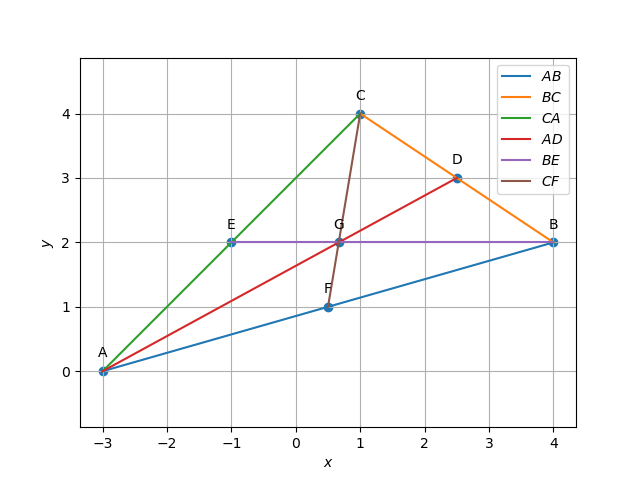
\includegraphics[width=\columnwidth]{/sdcard/geometry/geometry/figs/med2.png}
\caption{$G$ is the centroid of triangle $ABC$}
\label{fig:Triangle101}
\end{figure}



%Question 1.2.4:
\item Verify that 
		\begin{align}
			\frac{BG}{GE} = 
			\frac{CG}{GF} =
			\frac{AG}{GD} =2 
		\end{align}\\
Question 1.2.4:Verify that 
\begin{align}
		\frac{BG}{GE} = 
		\frac{CG}{GF} =
		\frac{AG}{GD} = 2 
\end{align}
\solution In order to verify the above equation we first need to find $\vec{G}$.$\vec{G}$ is the intersection of $BE$ and $CF$,Using the value of $\vec{G}$ from (1.2.3).
\begin{align}
		\vec{G} = \myvec{\frac{2}{3}\\2}
\end{align}
Also,We know that $\vec{D}, \vec{E}$ and $\vec{F}$ are midpoints of $BC, CA$ and $AB$ respectively from (1.2.1).
\begin{align}
		\vec{D} = \myvec{\frac{5}{2} \\ 3},\,
		\vec{E} = \myvec{-1 \\ 2},\,
		\vec{F} = \myvec{\frac{1}{2}\\ 1}
\end{align}
\begin{enumerate}
\item Calculating the ratio of $BG$ and $GE$,
\begin{align}
		\label{eq:tri-pts/4} \vec{G}-\vec{B} &= \myvec{\frac{-10}{3} \\ 0} \\
		\label{eq:tri-pts/5} \vec{E}-\vec{G} &= \myvec{\frac{-5}{3} \\ 0} \\
		\label{eq:tri-pts/6} \norm{\vec{G}-\vec{B}} &= \sqrt{\brak{\frac{-10}{0}}^2 + \brak{\frac{-5}{0}}^{2}}  \\
		\label{eq:tri-pts/7} \norm{\vec{E}-\vec{G}} &= \sqrt{\brak{\frac{-13}{6}}^2 + \brak{\frac{-4}{3}}^2} &= \frac{\sqrt{233}}{6} \\
		\label{eq:tri-pts/8}\frac{BG}{GE} &= \frac{\norm{\vec{G}-\vec{B}}}{\norm{\vec{E}-\vec{G}}}&= 2  
\end{align}		
\end{enumerate}

From \eqref{eq:tri-pts/8}, \eqref{eq:tri-pts/13}, \eqref{eq:tri-pts/18}
\begin{align}
		\frac{BG}{GE} = 
		\frac{CG}{GF} =
		\frac{AG}{GD} = 2
\end{align}
Hence verified.



%Question 1.2.5:
\item Show that $\vec{A}, \vec{G}$ and $\vec{D}$ are collinear.\\
\solution 
Given that,
\begin{align}
    \vec{A} = \myvec{-3\\0}
    \quad
    \vec{B} &= \myvec{4\\2}
    \quad
    \vec{C} = \myvec{1\\4}
\end{align}
We need to show that points $\vec{A},\vec{D},\vec{G}$ are collinear.
From Problem 1.2.3 We know that, The point $\vec{G}$ is 
\begin{align}
    \vec{G} &=\myvec{\frac{2}{3}\\ 2}
\end{align}
And from Problem 1.2.1 We know that, The point $\vec{D}$ is 
\begin{align}
    \vec{D} &=\myvec{\frac{5}{2}\\ 3}
\end{align}
In Problem 1.1.3, There is a theorem/law mentioned i.e.,

Points $\vec{A},\vec{D},\vec{G}$ are defined to be collinear if 
\begin{align}
    \text{rank}\myvec{
    1 & 1 & 1\\
    \vec{A} & \vec{D} & \vec{G} \\
    } &= 2 
\end{align} 
Using the above law/Theorem Let
\begin{align}
    \vec{R}&=\myvec{
    1 & 1 & 1
    \\
    -3 & \frac{5}{2} & \frac{2}{3}
    \\
    0 & 3 & 2
    } 
\end{align} 
The matrix $\vec{R}$ can be row reduced as follows,
\begin{align}
    \label{eq:mat_row_operations}
    \myvec{
    1 & 1 & 1
    \\
    -3 & \frac{5}{2} & \frac{2}{3}
    \\
    0 & 3 & 2
    }
     \xleftrightarrow[]{}
    \myvec{
    1 & 1 & 1
    \\
    0 & 1 & \frac{2}{3}
    \\
    0 & 0 & 0
    }
\end{align}
Rank of above matrix is 2.\\
Hence, we proved that that points $\vec{A},\vec{D},\vec{G}$ are collinear.



%Question 1.2.6:
\item Verify that 
		\begin{align}
			\vec{G}=\frac{\vec{A}+\vec{B}+\vec{C}}{3}
		\end{align}
$\vec{G}$ is known as the {\em centroid} of $\triangle ABC$.\\
Verify that\\
\begin{align}
 \vec{G}=\frac{\vec{A}+\vec{B}+\vec{C}}{3}   
\end{align}
$\vec{G}$ is known as the \underline{centroid} of $\triangle$ABC 
SOLUTION:\\
let us first evaluate the R.H.S of the equation
\begin{equation}
\begin{split}
\label{eq:centroid}
    \vec{G}&= \frac{\myvec{-3\\0}+\myvec{4\\2}+\myvec{1\\4}}{3}\\   
     &= \myvec{\frac{2}{3}\\ 2}
\end{split}
\end{equation}
Hence verified.


%Question 1.2.7: 
\item Verify that 
		\begin{align}
\vec{A}-\vec{F}=\vec{E}-\vec{D}
		\end{align}
The quadrilateral $AFDE$ is defined to be a parallelogram.\\
Question : Verify that 
\begin{align}
	\vec{A}-\vec{F} = \vec{E}-\vec{D}
\end{align}
The quadrilateral $AFDE$ is defined to be parallelogram
\\ \solution 
Given that,
\begin{align}
    \vec{A} = \myvec{-3\\0}
    \quad
    \vec{B} &= \myvec{4\\2}
    \quad
    \vec{C} = \myvec{1\\4}
\end{align}
From Problem 1.2.1 We know that, The point $\vec{D},\vec{E},\vec{F}$ is 
\begin{align}
    \vec{D} = \myvec{\frac{5}{2}\\ 3 }
    \quad
    \vec{E} &= \myvec{-1\\2}
    \quad
    \vec{F} = \myvec{\frac{1}{2}\\ 1}
\end{align}
Evaluating the R.H.S of the equation
\begin{align}
    \vec{A}-\vec{F}&=\myvec{ \frac{-7}{2} \\ -1 }
\end{align} 
Evaluating the L.H.S of the equation
\begin{align}
    \vec{E}-\vec{D}&=\myvec{\frac{-7}{2} \\ -1 }
\end{align}
Hence verified that, R.H.S = L.H.S i.e.,
\begin{align}
	\vec{A}-\vec{F} = \vec{E}-\vec{D}
\end{align}
From the fig\ref{fig:Triangle}, It is verified that $AFDE$ is a parallelogram
\begin{figure}
\centering
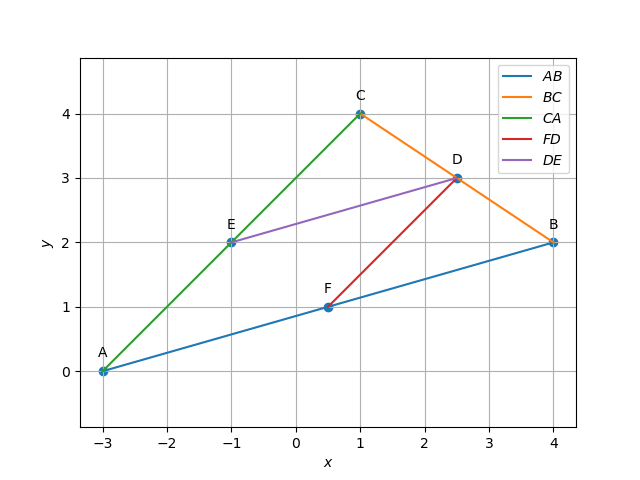
\includegraphics[width=\columnwidth]{/sdcard/geometry/geometry/figs/prm.png}
\caption{$AFDE$ form a parallelogram in triangle ABC}
\label{fig:Triangle}
\end{figure}
\end{enumerate}














%\documentclass[11pt]{book}
\usepackage{gvv-book}
\usepackage{gvv}
\usepackage[sectionbib,authoryear]{natbib}
\setcounter{secnumdepth}{3}
\setcounter{tocdepth}{2}
\makeindex

\begin{document}
\frontmatter
\tableofcontents
\setcounter{page}{1}
\mainmatter
\chapter{Triangle}
Consider a triangle with vertices
\begin{align}
\label{eq:tri-pts}
\vec{A}=\myvec{1 \\ 0},\,
\vec{B}=\myvec{5\\4},\,
	\vec{c}=\myvec{-4\\0},\,
\end{align}

\section{Vectors}
\section{median}


\begin{enumerate}[label=\thesection.\arabic*.,ref=\thesection.\theenumi]
\numberwithin{equation}{enumi}

%Question 1.2.1:
\item  If $\vec{D}$ divides $BC$ in the ratio $k : 1$,
		\begin{align}
			\vec{D}= \frac{k\vec{C}+\vec{B}}{k+1}
		\end{align}
Find the mid points $\vec{D}, \vec{E}, \vec{F}$ of the sides $BC, CA$ and $AB$ respectively.\\
If $\vec{D}$ divides $BC$ in the ratio $k : 1$,
\begin{align}
\vec{D}= \frac{k\vec{C}+\vec{B}}{k+1}
\end{align}
Find the mid points $\vec{D}, \vec{E}, \vec{F}$ of the sides $BC, CA$ and $AB$ respectively.
\newline
Given:
\begin{align}
\vec{A} &= \myvec{-3\\0\\}\\
\vec{B} &= \myvec{4\\2\\}\\
\vec{C} &= \myvec{1\\4\\}
\end{align}

\solution
Since $\vec{D}$ is the midpoint of $BC$,
\begin{align}
k &= 1\\
\implies \vec{D} &= \frac{\vec{C} + \vec{B}}{2}\\
&= \frac{1}{2}\myvec{5\\6}
\end{align}
Similarly,
\begin{align}
\vec{E} &= \frac{\vec{A} + \vec{C}}{2}\\
&= \frac{1}{2}\myvec{-2\\4}\\
\vec{F} &= \frac{\vec{A} + \vec{B}}{2}\\
&= \myvec{1/2\\1}
\end{align} 

%Question 1.2.2:
\item Find the equations of $AD, BE$ and $CF$.\\
\\ \solution:
$\vec{D}$,$\vec{E}$,$\vec{F}$ are the midpoints of $BC$,$CA$,$AB$ respectively, then\\
\begin{align}
 \vec{D} &=  \myvec{\frac{5}{2}\\3}\\
 \vec{E} &=  \myvec{-1\\2}\\
 \vec{F} &= \myvec{1/2\\1}
\end{align}
\begin{enumerate}

 \item The normal equation for the median $AD$ is
  \begin{align}
    \vec{n}^{\top}\myvec{\vec{x}-\vec{A}}&=0\\
    \implies
    \vec{n}^{\top}\vec{x}&=\vec{n}^{\top}\vec{A}
  \end{align}
 We have to find the $\vec{n}$ so that we can find $\vec{n}^{\top}$.
 Since,
\begin{align}
  \vec{n} &= \myvec{0 & 1\\
  -1 & 0}\vec{m}
\end{align}
Here $\vec{m} = \vec{D}- \vec{A}$ for median $AD$
\begin{align}
\vec{m}&=\myvec{\frac{11}{2}\\3}
\end{align}
Since,
\begin{align}
  \vec{n} &= \myvec{0 & 1\\
  -1 & 0}\vec{m}\\
\implies
\vec{n} &= \myvec{0 & 1\\
  -1 & 0}\myvec{\frac{11}{2}\\3}\\
        &= \myvec{3 \\\frac{-11}{2}}
\end{align}
Hence the normal equation of median $AD$ is 
\begin{align}
    \myvec{3 & \frac{-11}{2}}\vec{x}&=\myvec{3 & \frac{-11}{2}}\myvec{-3\\0}\\
    \implies
    \myvec{3 & \frac{-11}{2}}\vec{x}&={-9}
\end{align}

\item The normal equation for the median $BE$ is
\begin{align}
\vec{n}^{\top}\myvec{\vec{x}-\vec{B}}&=0\\
\implies
\vec{n}^{\top}\vec{x}&=\vec{n}^{\top}\vec{B}
\end{align}
Here $\vec{m} = \vec{E}- \vec{B}$ for median $BE$
\begin{align}
\vec{m}&&=\myvec{-5\\0}
\end{align}
Since,
\begin{align}
  \vec{n} &= \myvec{0 & 1\\
  -1 & 0}\vec{m}\\
\implies
\vec{n} &= \myvec{0 & 1\\
  -1 & 0}\myvec{-5\\0}\\
        &= \myvec{0\\ 5}
\end{align}
Hence the normal equation of median $BE$ is 
\begin{align}
    \myvec{0 & 5}\vec{x}&=\myvec{0 & 5}\myvec{4\\2}\\
\implies
    \myvec{0 & 5}\vec{x}&={10}
\end{align}

\item The normal equation for the median $CF$ is
\begin{align}
\vec{n}^{\top}\myvec{\vec{x}-\vec{C}}&=0\\
\implies
\vec{n}^{\top}\vec{x}&=\vec{n}^{\top}\vec{C}
\end{align}
Here $\vec{m} = \vec{F}- \vec{C}$ for median $CF$
\begin{align}
\vec{m}&=\myvec{\frac{-1}{2}\\-3}
\end{align}
Since,
\begin{align}
  \vec{n} &= \myvec{0 & 1\\
  -1 & 0}\vec{m}\\
\implies
\vec{n} &= \myvec{0 & 1\\
  -1 & 0}\myvec{\frac{-1}{2} \\ -3 }\\
        &= \myvec{-3 \\ \frac{1}{2}}
\end{align}
Hence the normal equation of median $CF$ is 
\begin{align}
    \myvec{-3 & \frac{1}{2} }\vec{x}&=\myvec{-3 & \frac{1}{2}}\myvec{1\\4}\\
\implies
    \myvec{-3 & \frac{1}{2}}\vec{x}&=-1
\end{align}
\end{enumerate}

%Question 1.2.3:
\item Find the intersection $\vec{G}$ of $BE$ and $CF$
\\ 
\solution 
$\vec{A},\vec{B}$ and $\vec{C}$ are vertices of triangle:
\begin{align}
    \vec{A} &= \myvec-3 \\0} \\
    \vec{B} &= \myvec{4\\ 2} \\
    \vec{C} &= \myvec{1 \\4}
\end{align}
Since $\vec{E}$ and $\vec{F}$ are midpoints of $CA$ and $AB$,
\begin{align}
    \vec{E} &= \frac{\vec{A} + \vec{C}}{2} \\
	&= \myvec{-1 \\2}\\
    \vec{F} &= \frac{\vec{B} + \vec{A}}{2} \\ 
    &= \myvec{ \frac{1}{2} \\ 1}
\end{align}
The line $BE$ in vector form is given by
\begin{align}
\myvec{0 & 5} \vec{x} &= \myvec{10}
\label{eq:1.2.3,8}
\end{align}
The line $CF$ in vector form is given by
\begin{align}
\myvec{ -3&-\frac{1}{2}} \vec{x} &= \myvec{-1}
\label{eq:1.2.3,9}
\end{align}
From \eqref{eq:1.2.3,8} and \eqref{eq:1.2.3,9} the augmented matrix is:
\begin{align}
\myvec{
0 & 5 & {10} \\
-3 & \frac{1}{2} & -1
}
\end{align}
Solve for $\vec{x}$ using Gauss-Elimination method:
\begin{align}
    \label{eq:matrowoperations}
    \myvec{
    1 & 0 & \frac{2}{3}
    \\
    0 & 1 & 2
    }
\end{align} 
Therefore, 
\begin{align}
\vec{G} = \myvec{\frac{2}{3} \\ 2}
\end{align}
From Fig. \ref{fig:Triangle101}, We can see that $\vec{G}=\myvec{\frac{2}{3}\\ 2}$ is the intersection of $BE$ and $CF$
\begin{figure}[h]
\centering
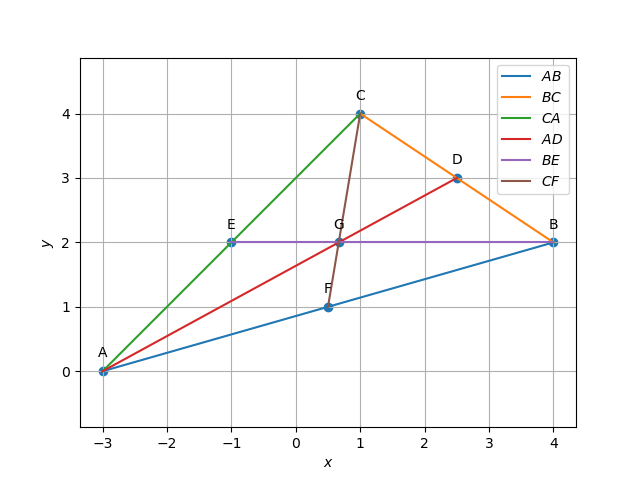
\includegraphics[width=\columnwidth]{/sdcard/geometry/geometry/figs/med2.png}
\caption{$G$ is the centroid of triangle $ABC$}
\label{fig:Triangle101}
\end{figure}



%Question 1.2.4:
\item Verify that 
		\begin{align}
			\frac{BG}{GE} = 
			\frac{CG}{GF} =
			\frac{AG}{GD} =2 
		\end{align}\\
Question 1.2.4:Verify that 
\begin{align}
		\frac{BG}{GE} = 
		\frac{CG}{GF} =
		\frac{AG}{GD} = 2 
\end{align}
\solution In order to verify the above equation we first need to find $\vec{G}$.$\vec{G}$ is the intersection of $BE$ and $CF$,Using the value of $\vec{G}$ from (1.2.3).
\begin{align}
		\vec{G} = \myvec{\frac{2}{3}\\2}
\end{align}
Also,We know that $\vec{D}, \vec{E}$ and $\vec{F}$ are midpoints of $BC, CA$ and $AB$ respectively from (1.2.1).
\begin{align}
		\vec{D} = \myvec{\frac{5}{2} \\ 3},\,
		\vec{E} = \myvec{-1 \\ 2},\,
		\vec{F} = \myvec{\frac{1}{2}\\ 1}
\end{align}
\begin{enumerate}
\item Calculating the ratio of $BG$ and $GE$,
\begin{align}
		\label{eq:tri-pts/4} \vec{G}-\vec{B} &= \myvec{\frac{-10}{3} \\ 0} \\
		\label{eq:tri-pts/5} \vec{E}-\vec{G} &= \myvec{\frac{-5}{3} \\ 0} \\
		\label{eq:tri-pts/6} \norm{\vec{G}-\vec{B}} &= \sqrt{\brak{\frac{-10}{0}}^2 + \brak{\frac{-5}{0}}^{2}}  \\
		\label{eq:tri-pts/7} \norm{\vec{E}-\vec{G}} &= \sqrt{\brak{\frac{-13}{6}}^2 + \brak{\frac{-4}{3}}^2} &= \frac{\sqrt{233}}{6} \\
		\label{eq:tri-pts/8}\frac{BG}{GE} &= \frac{\norm{\vec{G}-\vec{B}}}{\norm{\vec{E}-\vec{G}}}&= 2  
\end{align}		
\end{enumerate}

From \eqref{eq:tri-pts/8}, \eqref{eq:tri-pts/13}, \eqref{eq:tri-pts/18}
\begin{align}
		\frac{BG}{GE} = 
		\frac{CG}{GF} =
		\frac{AG}{GD} = 2
\end{align}
Hence verified.



%Question 1.2.5:
\item Show that $\vec{A}, \vec{G}$ and $\vec{D}$ are collinear.\\
\solution 
Given that,
\begin{align}
    \vec{A} = \myvec{-3\\0}
    \quad
    \vec{B} &= \myvec{4\\2}
    \quad
    \vec{C} = \myvec{1\\4}
\end{align}
We need to show that points $\vec{A},\vec{D},\vec{G}$ are collinear.
From Problem 1.2.3 We know that, The point $\vec{G}$ is 
\begin{align}
    \vec{G} &=\myvec{\frac{2}{3}\\ 2}
\end{align}
And from Problem 1.2.1 We know that, The point $\vec{D}$ is 
\begin{align}
    \vec{D} &=\myvec{\frac{5}{2}\\ 3}
\end{align}
In Problem 1.1.3, There is a theorem/law mentioned i.e.,

Points $\vec{A},\vec{D},\vec{G}$ are defined to be collinear if 
\begin{align}
    \text{rank}\myvec{
    1 & 1 & 1\\
    \vec{A} & \vec{D} & \vec{G} \\
    } &= 2 
\end{align} 
Using the above law/Theorem Let
\begin{align}
    \vec{R}&=\myvec{
    1 & 1 & 1
    \\
    -3 & \frac{5}{2} & \frac{2}{3}
    \\
    0 & 3 & 2
    } 
\end{align} 
The matrix $\vec{R}$ can be row reduced as follows,
\begin{align}
    \label{eq:mat_row_operations}
    \myvec{
    1 & 1 & 1
    \\
    -3 & \frac{5}{2} & \frac{2}{3}
    \\
    0 & 3 & 2
    }
     \xleftrightarrow[]{}
    \myvec{
    1 & 1 & 1
    \\
    0 & 1 & \frac{2}{3}
    \\
    0 & 0 & 0
    }
\end{align}
Rank of above matrix is 2.\\
Hence, we proved that that points $\vec{A},\vec{D},\vec{G}$ are collinear.



%Question 1.2.6:
\item Verify that 
		\begin{align}
			\vec{G}=\frac{\vec{A}+\vec{B}+\vec{C}}{3}
		\end{align}
$\vec{G}$ is known as the {\em centroid} of $\triangle ABC$.\\
Verify that\\
\begin{align}
 \vec{G}=\frac{\vec{A}+\vec{B}+\vec{C}}{3}   
\end{align}
$\vec{G}$ is known as the \underline{centroid} of $\triangle$ABC 
SOLUTION:\\
let us first evaluate the R.H.S of the equation
\begin{equation}
\begin{split}
\label{eq:centroid}
    \vec{G}&= \frac{\myvec{-3\\0}+\myvec{4\\2}+\myvec{1\\4}}{3}\\   
     &= \myvec{\frac{2}{3}\\ 2}
\end{split}
\end{equation}
Hence verified.


%Question 1.2.7: 
\item Verify that 
		\begin{align}
\vec{A}-\vec{F}=\vec{E}-\vec{D}
		\end{align}
The quadrilateral $AFDE$ is defined to be a parallelogram.\\
Question : Verify that 
\begin{align}
	\vec{A}-\vec{F} = \vec{E}-\vec{D}
\end{align}
The quadrilateral $AFDE$ is defined to be parallelogram
\\ \solution 
Given that,
\begin{align}
    \vec{A} = \myvec{-3\\0}
    \quad
    \vec{B} &= \myvec{4\\2}
    \quad
    \vec{C} = \myvec{1\\4}
\end{align}
From Problem 1.2.1 We know that, The point $\vec{D},\vec{E},\vec{F}$ is 
\begin{align}
    \vec{D} = \myvec{\frac{5}{2}\\ 3 }
    \quad
    \vec{E} &= \myvec{-1\\2}
    \quad
    \vec{F} = \myvec{\frac{1}{2}\\ 1}
\end{align}
Evaluating the R.H.S of the equation
\begin{align}
    \vec{A}-\vec{F}&=\myvec{ \frac{-7}{2} \\ -1 }
\end{align} 
Evaluating the L.H.S of the equation
\begin{align}
    \vec{E}-\vec{D}&=\myvec{\frac{-7}{2} \\ -1 }
\end{align}
Hence verified that, R.H.S = L.H.S i.e.,
\begin{align}
	\vec{A}-\vec{F} = \vec{E}-\vec{D}
\end{align}
From the fig\ref{fig:Triangle}, It is verified that $AFDE$ is a parallelogram
\begin{figure}
\centering
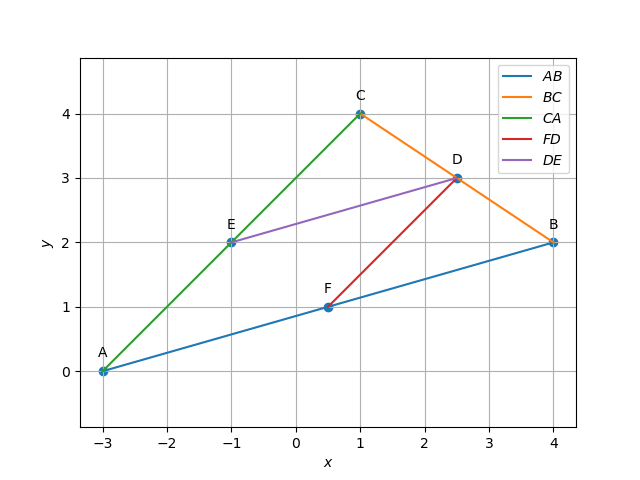
\includegraphics[width=\columnwidth]{/sdcard/geometry/geometry/figs/prm.png}
\caption{$AFDE$ form a parallelogram in triangle ABC}
\label{fig:Triangle}
\end{figure}
\end{enumerate}














%\input{subsec/median}
%\section{Altitude}
%\section{Perpendicular Bisector}
%\section{Angle Bisector}

\end{document}
{

%\section{Altitude}
%\section{Perpendicular Bisector}
%\section{Angle Bisector}

\end{document}
{

%\section{Altitude}
%\section{Perpendicular Bisector}
%\section{Angle Bisector}

\end{document}
{

%\section{Altitude}
%\section{Perpendicular Bisector}
%\section{Angle Bisector}

\end{document}
{
